\documentclass[11pt,a4paper]{article}
\usepackage[margin=25mm]{geometry}
\usepackage[T1]{fontenc}
\usepackage{amsmath,amssymb,bm}
\usepackage{graphicx}
\usepackage{booktabs}
\usepackage{tabularx}
\usepackage{tikz}
\usetikzlibrary{arrows.meta,positioning,calc}
\usepackage[round]{natbib}
\usepackage{hyperref}
\hypersetup{colorlinks=true, urlcolor=blue, linkcolor=blue, citecolor=blue}

\newcommand{\code}[1]{\texttt{#1}}
\newcommand{\dd}{\mathrm{d}}

\title{Benchmarking guiding-centre orbits in axisymmetric tokamak fields:\\
SIMPLE versus POTATO}
\author{Plasma group, Institute of Theoretical and Computational Physics,
TU Graz}
\date{July 2026, working document}

\begin{document}
\maketitle

\begin{abstract}
SIMPLE and POTATO both integrate collisionless guiding-centre orbits in
toroidal magnetic fields, with different numerics: SIMPLE uses symplectic
integrators in canonical coordinates, POTATO an adaptive
Runge--Kutta scheme in cylindrical coordinates with event-based orbit closure.
In an axisymmetric tokamak field both solve the same integrable problem, so
every observable of a single orbit is directly comparable: conserved
quantities, bounce and transit frequency, toroidal precession, orbit width,
and Poincar\'e sections. This document fixes the coordinate and pitch
conventions, common field, estimators, and acceptance criteria. NEO-RT
thin-orbit frequencies provide a third reference. The repository work plan
gives the executable procedure and current status; the Rung 0 README gives the
input manifest.
\end{abstract}

\section{Purpose}

A tokamak field with nested flux surfaces makes guiding-centre motion
integrable: three independent invariants exist, orbits are closed in the
poloidal plane, and each orbit carries well-defined frequencies. Two codes
that integrate the same equations must therefore agree on every orbit
observable up to their discretisation errors, which have known and very
different structure in the two cases. Agreement across the trapped--passing
boundary and in the near-axis region, where orbit widths are largest, is a
verification result that neither code currently has against the other.
Disagreement that survives resolution scans localises a defect. The common
field, frequency extraction, and orbit overlays can then be reused for later
orbit-code benchmarks.

The scope is axisymmetric, unperturbed,
collisionless, static fields, single-particle observables. Perturbed fields,
transport coefficients, and stellarator geometry are not treated here;
Section~\ref{sec:outlook} points to where they connect.

\section{Guiding-centre motion in an axisymmetric tokamak}
\label{sec:theory}

\subsection{Field, coordinates, units}

We use Gaussian units throughout, matching both codes. Cylindrical
coordinates are $(R,\varphi,Z)$ with major radius $R$, toroidal angle
$\varphi$, and vertical coordinate $Z$. An axisymmetric equilibrium field is
\begin{equation}
  \bm B \;=\; \nabla\psi \times \nabla\varphi \;+\; B_\varphi\, R\,\nabla\varphi ,
  \label{eq:field}
\end{equation}
where $\psi(R,Z)$ is the poloidal flux function (poloidal flux divided by
$2\pi$) and $B_\varphi R = F(\psi)$ is the covariant toroidal field component,
a flux function in equilibrium. The safety factor $q(\psi)$ is the number of
toroidal turns per poloidal turn of a field line. For estimates we use the
large-aspect-ratio circular model
\begin{equation}
  B \;\approx\; B_0\,\bigl(1 - \varepsilon\cos\theta\bigr),
  \qquad \varepsilon = r/R_0 \ll 1,
  \label{eq:Bcirc}
\end{equation}
with minor radius $r$ of the flux surface, magnetic axis at $R_0$, poloidal
angle $\theta$ counted from the outboard midplane, and field strength $B_0$
on axis.

\subsection{Equations of motion and invariants}

A guiding centre with mass $m$, charge $e$, velocity modulus $v$, parallel
velocity $v_\parallel$, and perpendicular velocity $v_\perp$ carries the
magnetic moment
\begin{equation}
  \mu \;=\; \frac{m v_\perp^2}{2B}.
\end{equation}
In guiding-centre theory $\mu$ is an adiabatic invariant of the underlying
particle motion; within the guiding-centre model itself it enters as an exact
parameter \citep{littlejohn1983}. The Hamiltonian for a static field without
electric potential is
\begin{equation}
  H \;=\; \frac{m v_\parallel^2}{2} + \mu B \;=\; \frac{m v^2}{2} \;=\; E,
  \label{eq:H}
\end{equation}
the kinetic energy. Axisymmetry makes $\varphi$ cyclic, so the canonical
toroidal momentum is conserved. In the form used by POTATO,
\begin{equation}
  \psi^* \;\equiv\; \frac{c}{e}\,p_\varphi
  \;=\; \psi \;+\; \frac{m c}{e}\, v_\parallel\, \frac{B_\varphi R}{B},
  \label{eq:pphi}
\end{equation}
which reduces to the flux label $\psi$ in the zero-orbit-width limit. The
three quantities $(E, \mu, p_\varphi)$ are exact invariants of the
guiding-centre flow in an axisymmetric field. Two distinct roles follow for
the benchmark:
\begin{itemize}
\item $\mu$ is a \emph{parameter} of the guiding-centre equations. Both codes
  keep it constant to machine precision by construction; its drift is not a
  discriminating metric for guiding-centre runs. It becomes a real metric only
  in full-orbit (gyro-resolved) integration, which SIMPLE offers as an
  optional cross-check.
\item $E$ and $p_\varphi$ are \emph{dynamical} invariants that the integrator
  must preserve numerically. Their drift over long traces is the primary
  numerical-quality metric, and this is where symplectic and non-symplectic
  schemes differ qualitatively: symplectic schemes bound the energy error over
  exponentially long times, adaptive non-symplectic schemes accumulate a
  secular drift controlled by the local tolerance \citep{albert2020jcp}.
\end{itemize}

\subsection{Orbit classes}
\label{sec:classes}

Define the pitch cosine at the outboard midplane of a flux surface as
$\xi_0 = v_\parallel(\theta{=}0)/v$. The analytic trapping parameter is
$\Lambda = \mu B_0/E$. For a given surface they are related by
\begin{equation}
  \Lambda = (1-\xi_0^2)\,\frac{B_0}{B(\theta=0)}.
\end{equation}
The code inputs use $\xi$, while the analytic formulas below use $\Lambda$.
In the circular model \eqref{eq:Bcirc} the parallel velocity along the orbit is
\begin{equation}
  v_\parallel^2 \;=\; v^2\,\bigl[\,1 - \Lambda\,(1-\varepsilon\cos\theta)\,\bigr].
\end{equation}
A particle is trapped when $v_\parallel$ vanishes at some $\theta_t$ before
completing a poloidal turn, i.e.\ for
$1/(1+\varepsilon) < \Lambda < 1/(1-\varepsilon)$; otherwise it is passing.
The boundary between the two classes, the trapped--passing separatrix, is a
codimension-one surface in $(\Lambda,\varepsilon)$; the bounce time diverges
logarithmically as it is approached, which makes it the numerically hardest
region and therefore a mandatory part of every scan in this benchmark.

Finite orbit width adds structure near the magnetic axis: when the poloidal
gyration width becomes comparable to the distance from the axis, trapped
orbits deform into \emph{potato} orbits that enclose the axis. POTATO resolves
this class numerically; SIMPLE also integrates the finite-width guiding-centre
orbit. The near-axis region is therefore part of the comparison.
Figure~\ref{fig:orbits} sketches the three classes.

\begin{figure}[htb]
\centering
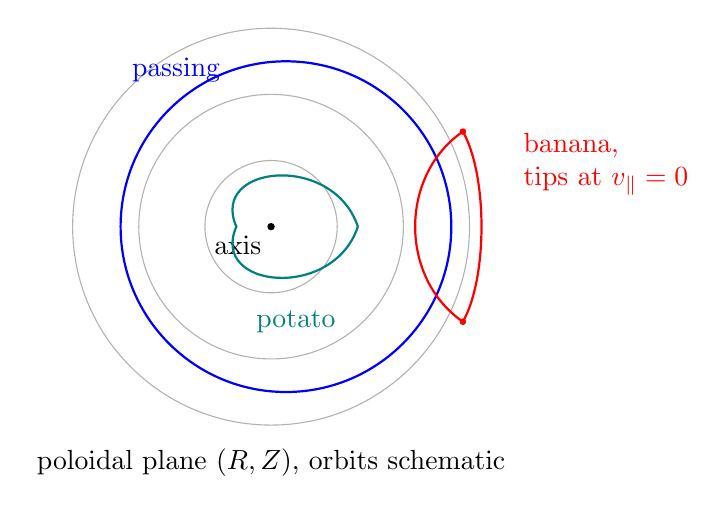
\begin{tikzpicture}[scale=1.05]
  % flux surfaces
  \draw[gray!60] (0,0) circle (2.4);
  \draw[gray!60] (0,0) circle (1.6);
  \draw[gray!60] (0,0) circle (0.8);
  \fill (0,0) circle (0.045) node[below left] {axis};
  % passing orbit: slightly shifted circle
  \draw[thick,blue] (0.18,0) circle (2.0);
  \node[blue] at (-1.15,1.9) {passing};
  % banana: crescent on outboard side
  \draw[thick,red]
    (2.32,1.15) .. controls (1.55,0.62) and (1.55,-0.62) .. (2.32,-1.15)
    .. controls (2.62,-0.62) and (2.62,0.62) .. (2.32,1.15);
  \fill[red] (2.32,1.15) circle (0.04);
  \fill[red] (2.32,-1.15) circle (0.04);
  \node[red,align=left] at (4.05,0.75) {banana,\\tips at $v_\parallel=0$};
  % potato: teardrop enclosing axis
  \draw[thick,teal]
    (1.05,0) .. controls (0.75,0.9) and (-0.75,0.75) .. (-0.42,0)
    .. controls (-0.75,-0.75) and (0.75,-0.9) .. (1.05,0);
  \node[teal] at (0.3,-1.15) {potato};
  \node at (0,-2.85) {poloidal plane $(R,Z)$, orbits schematic};
\end{tikzpicture}
\caption{Guiding-centre orbit classes in the poloidal plane. Passing orbits
encircle the axis close to a flux surface, banana orbits are trapped on the
outboard side with turning points where $v_\parallel = 0$, and potato orbits
arise near the axis where the orbit width is comparable to the distance from
the axis.}
\label{fig:orbits}
\end{figure}

\subsection{Canonical frequencies}
\label{sec:frequencies}

Integrability provides action-angle variables, and with them two frequencies
per orbit \citep{albert2016}:
\begin{align}
  \omega_b &= \frac{2\pi}{\tau_b},
  &&\text{bounce (trapped) or transit (passing) frequency,} \\
  \omega_\varphi &= \frac{\Delta\varphi_b}{\tau_b},
  &&\text{mean toroidal precession frequency,}
\end{align}
where $\tau_b$ is the time for one closed poloidal cycle and
$\Delta\varphi_b$ the toroidal angle accumulated during it. For passing
particles $\Delta\varphi_b \approx 2\pi q$ plus a drift correction; for
trapped particles $\Delta\varphi_b$ is the net precession per bounce. Every
resonance condition of perturbed transport theory is a linear
integer combination $m\,\omega_b + n\,\omega_\varphi$, which stays finite and
smooth across the trapped--passing boundary even though $\tau_b$ and
$\Delta\varphi_b$ individually diverge there. Comparing $\omega_b$ and
$\omega_\varphi$ between codes therefore tests the quantities that
downstream applications consume.

For the circular model, standard large-aspect-ratio expressions exist in
terms of complete elliptic integrals $K(\kappa)$ and $E(\kappa)$ with
\begin{equation}
  \kappa^2 \;=\; \frac{1-\Lambda(1-\varepsilon)}{2\,\varepsilon\Lambda},
\end{equation}
$\kappa^2 \in (0,1)$ for trapped orbits: the deeply trapped bounce frequency
$\omega_b \to \sqrt{\varepsilon\Lambda/2}\;v/(qR_0)\cdot
\pi/(2K(\kappa))\big|_{K(0)=\pi/2}$, and a trapped precession of the form
$\omega_\varphi \propto \bigl(2E(\kappa)/K(\kappa)-1\bigr)$ with magnetic-shear
corrections; see \citet{helander2002} for the derivation and conventions.
These formulas serve as sanity envelopes for rung~2 of the work plan. Because
convention factors of order $\Lambda \approx 1$ differ between references,
they must be re-derived in the chosen normalisation before being used as
quantitative acceptance bounds; until then, code-versus-code agreement is the
primary criterion and the analytic forms bound the plausible range.

\subsection{Orbit width}

The radial excursion of a banana orbit at the midplane, the banana width, is
in the circular model
\begin{equation}
  \Delta_b \;\sim\; \frac{q\,\rho}{\sqrt{\varepsilon}},
  \qquad \rho = \frac{m c\, v}{e B},
  \label{eq:width}
\end{equation}
up to a factor of order unity depending on $\kappa$. The width is directly
measurable in both codes from the $(R,Z)$ footprint of one closed orbit and,
unlike the frequencies, requires no time information, so it cross-checks the
orbit geometry before any clock enters the comparison. Near the axis, where
\eqref{eq:width} formally exceeds the distance to the axis, the banana picture
gives way to the potato class and the width must be compared numerically
rather than against the estimate.

\subsection{Poincar\'e sections}
\label{sec:poincare}

A Poincar\'e section reduces the continuous orbit to a discrete map: record
the phase-space point each time the orbit crosses a chosen surface of
section in a fixed direction. The benchmark uses two sections:
\begin{itemize}
\item the \emph{tip section} $v_\parallel = 0$ for trapped orbits (banana
  tips), and
\item a \emph{toroidal section} $\varphi = \mathrm{const}$ (modulo the field
  period).
\end{itemize}
In an axisymmetric field every orbit is a single closed curve in the poloidal
plane, so its section is a finite set of points; numerical non-conservation
smears these points into small islands or drifting clusters, which makes the
section a sensitive visual and quantitative diagnostic. The same section
definitions apply to perturbed and three-dimensional fields, where the point
set distinguishes regular from chaotic orbits.

\section{The codes}
\label{sec:codes}

\subsection{SIMPLE}

SIMPLE \citep{albert2020jcp} integrates guiding-centre orbits with symplectic
schemes formulated in canonical straight-field-line coordinates
\citep{albert2025}. Field input is a flux-coordinate description: VMEC
equilibria or a Boozer chart map (a NetCDF file tabulating the coordinate
chart and field on a grid). The state vector is
$z = (s, \theta, \varphi, p, \xi)$ with normalised toroidal flux $s$,
poloidal and toroidal angles, momentum modulus $p$, and pitch
$\xi = v_\parallel/v$. The integrator state carries the canonical pair
including $p_\varphi$ directly, so $H$ and $p_\varphi$ can be evaluated along
the trace and their numerical drift measured. Available schemes range
from explicit-implicit Euler through midpoint to Gauss and Lobatto
Runge--Kutta variants; a fourth-order Runge--Kutta reference and an optional
gyro-resolved full-orbit (Boris) pusher exist for cross-checks. The main
program traces particle ensembles with OpenMP parallelism and writes loss
times, confined fractions, orbit classification, reference coordinates, and
direct cylindrical $R,Z$ trajectory variables. The latter are evaluated
through the active VMEC or chart-map geometry and carry a NetCDF unit
attribute. A Python layer
(\code{pysimple}, built on f90wrap \citep{kermode2020}) exposes batch tracing
where one call integrates $N$ particles for a full trace time, so no
per-timestep call overhead occurs at the language boundary.

Current limitations, reviewed on 2026-07-10 and tracked in
\code{WORKPLAN.md}: the trajectory example works through
\code{pysimple.trace\_orbit}, but the dedicated Poincar\'e-cut routine has no
wrapped public driver; bounce and precession frequencies are not computed by
SIMPLE; and SIMPLE has no direct EQDSK input path. Orbit classification uses
an independent in-code implementation of tip and period detection.

\subsection{POTATO}

POTATO computes finite-orbit-width guiding-centre orbits in cylindrical
coordinates directly from an EFIT g-file (EQDSK), read through the shared
library libneo. The state vector is $z=(R,\varphi,Z,p,\xi)$. POTATO retains
the historical input name \code{orbit\_lambda} for $\xi=v_\parallel/v$.
Integration
uses an adaptive Runge--Kutta--Cash--Karp scheme; one closed poloidal cycle is
detected by crossings of a precomputed reference curve (the line where
$\nabla\psi\times\nabla B$ vanishes, reducing to the midplane in up-down
symmetric fields) followed by a Newton refinement that closes the orbit to a
relative tolerance of $10^{-10}$. The primitive \code{find\_bounce} returns
the bounce time $\tau_b$, the toroidal shift $\Delta\varphi_b$ per cycle, and
optional bounce integrals for a caller-supplied right-hand side; from these
the code derives $\omega_b$ and $\omega_\varphi$ in a built-in radial
frequency scan mode and in an $\eta$-scan diagnostic that tabulates
$\omega_b$ and $\Omega_{\mathrm{tor}}$ against the perpendicular invariant
for both signs of $v_\parallel$. Orbit classes including potatoes and the
trapped--passing boundary are resolved by a dedicated classification module
built on a first-return map. Invariants enter as parameters
$(E, \mu\text{-like perpendicular invariant}, \mathrm{sgn}\,v_\parallel)$,
and $\psi^*$ \eqref{eq:pphi} is evaluated along orbits by a dedicated
routine, so the $p_\varphi$ drift is directly accessible.

POTATO ships a public synthetic circular-tokamak test case (generated
g-file, no experimental data) used as a golden-record regression, which this
benchmark adopts as its common field, and has no Python bindings at present.

\subsection{NEO-RT thin-orbit frequencies as a third reference}

NEO-RT \citep{albert2016} computes resonant transport from thin-orbit
(zero-width) bounce-averaged dynamics on flux surfaces, with canonical
frequencies $\omega_b$ and $\omega_\varphi$ evaluated from one-dimensional
bounce integrals and splined over pitch. In the limit of small orbit width
the finite-width frequencies of POTATO and SIMPLE must converge to the
NEO-RT values, with deviations scaling with the orbit width itself. That
gives the frequency comparison a three-way structure: two finite-width codes
against each other at equal physics, and both against the thin-orbit limit
with a known convergence direction. A first comparison driver on the NEO-RT
side (a flux-surface scan at fixed pitch and energy writing the same columns
as POTATO's frequency scan) already exists in the NEO-RT test tree.

\subsection{Feature summary}

\begin{table}[htb]
\centering
\small
\begin{tabularx}{\textwidth}{@{}lXXX@{}}
\toprule
 & SIMPLE & POTATO & NEO-RT (thin orbit) \\
\midrule
orbit model & finite width, GC & finite width, GC & zero width, bounce avg. \\
coordinates & canonical flux; direct $R,Z$ output & cylindrical $(R,\varphi,Z)$ & flux surface label \\
integrator & symplectic (var.) & adaptive RK45 & adaptive Adams (VODE) \\
orbit closure & none (time stepping) & section crossing + Newton & turn event detection \\
field input & VMEC, Boozer chartmap & EQDSK via libneo & Boozer text / chartmap \\
$\omega_b,\ \omega_\varphi$ & absent (to be added) & native scan modes & native, splined \\
Poincar\'e cuts & wrapped driver pending & section infrastructure & n/a \\
potato class & carried implicitly & resolved and classified & outside model \\
Python layer & \code{pysimple} (f90wrap) & none & none \\
parallelism & OpenMP (+ GPU exp.) & OpenMP & OpenMP \\
\bottomrule
\end{tabularx}
\caption{Capabilities relevant to this benchmark, as of July 2026.}
\label{tab:features}
\end{table}

\section{Benchmark definition}
\label{sec:benchmark}

\subsection{Common field}
\label{sec:field}

Both codes use representations of the same synthetic circular equilibrium.
Their interpolation mismatch must be measured before it can be separated from
an orbit-integration difference. The tracked inputs are:
\begin{itemize}
\item POTATO reads \code{rung0/potato\_run/circ.eqdsk}, a byte-identical copy
  of its public synthetic golden-record equilibrium.
\item SIMPLE reads \code{rung0/circ\_chartmap\_simple.nc}. It was produced
  from that EQDSK with libneo's merged EQDSK-to-Boozer converter, then
  resampled onto SIMPLE's axis-complete uniform grid. Geometry is in
  centimetres and the radial coordinate is
  $\rho_{\mathrm{tor}}=\sqrt{s_{\mathrm{tor}}}$.
\end{itemize}
Do not use SIMPLE's built-in analytic test field
(\code{isw\_field\_type = -1}); it is a different hardcoded circular field.
The representation error is measured before any orbit comparison by
sampling $B$ and $\psi$ of both representations along matched $(R,Z)$ points
(rung~1 of the work plan). The complete file manifest and generation chain are
in \code{rung0/README.md}.

\begin{figure}[htb]
\centering
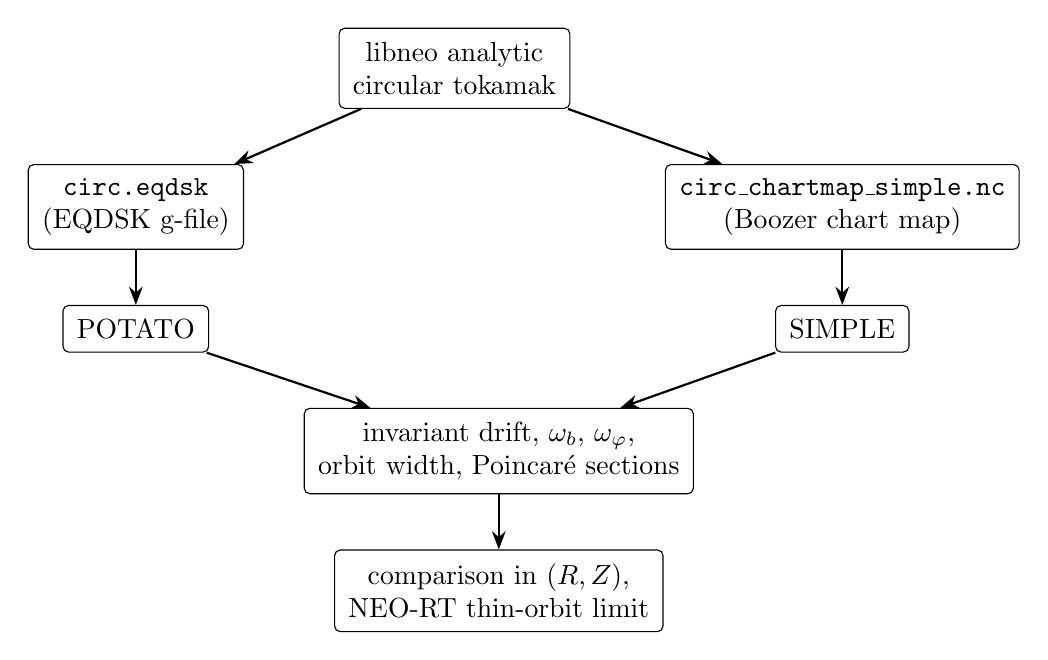
\begin{tikzpicture}[
  node distance=7mm and 12mm,
  box/.style={draw, rounded corners=2pt, align=center, inner sep=5pt},
  arr/.style={-{Stealth}, thick}
]
  \node[box] (libneo) {libneo analytic\\circular tokamak};
  \node[box, below left=of libneo] (eqdsk) {\code{circ.eqdsk}\\(EQDSK g-file)};
  \node[box, below right=of libneo] (chart) {
    \code{circ\_chartmap\_simple.nc}\\(Boozer chart map)};
  \node[box, below=of eqdsk] (potato) {POTATO};
  \node[box, below=of chart] (simple) {SIMPLE};
  \node[box, below right=of potato] (metrics) {invariant drift, $\omega_b$, $\omega_\varphi$,\\
    orbit width, Poincar\'e sections};
  \node[box, below=of metrics] (cmp) {comparison in $(R,Z)$,\\NEO-RT thin-orbit limit};
  \draw[arr] (libneo) -- (eqdsk);
  \draw[arr] (libneo) -- (chart);
  \draw[arr] (eqdsk) -- (potato);
  \draw[arr] (chart) -- (simple);
  \draw[arr] (potato) -- (metrics);
  \draw[arr] (simple) -- (metrics);
  \draw[arr] (metrics) -- (cmp);
\end{tikzpicture}
\caption{Benchmark pipeline. One analytic field feeds both codes through
their native input formats; all metrics are compared in cylindrical
coordinates.}
\label{fig:pipeline}
\end{figure}

\subsection{Reference particle and sweeps}

The reference particle is a deuteron ($A=2$, $Z=1$) at $E = 5\,$keV, taken
from the POTATO golden-record case so that its profiles are reused unchanged.
We run three one-dimensional sweeps:
\begin{enumerate}
\item \textbf{Radial}: select $\rho_{\mathrm{pol}}$ on the EQDSK side and
  match the same physical surface on the chart-map side. Do not identify
  POTATO's $\rho_{\mathrm{pol}}$ numerically with SIMPLE's
  $\rho_{\mathrm{tor}}$. Scan from near-axis to near-edge at fixed pitch.
\item \textbf{Pitch}: $\xi=v_\parallel/v$ through the trapped--passing
  boundary at fixed surface and energy, with points clustered toward the
  separatrix where $\tau_b$ diverges logarithmically.
\item \textbf{Energy}: widening the orbit width at fixed surface and pitch,
  from 1\,keV until potato or loss physics intervenes. This sweep controls the
  convergence toward the NEO-RT thin-orbit limit.
\end{enumerate}

\subsection{Metrics and estimators}
\label{sec:metrics}

For one orbit at a fixed physical surface, pitch cosine $\xi$, and energy $E$:
\begin{enumerate}
\item \textbf{Invariant drift}: relative drift of $E$ and $p_\varphi$
  (via $\psi^*$) over the trace, reported against trace length and step count.
  $\mu$ drift is reported only for the optional full-orbit cross-check runs.
\item \textbf{Frequencies}: $\omega_b$ and $\omega_\varphi$.
  POTATO: native (\code{find\_bounce}-based scan modes).
  NEO-RT: native splined thin-orbit values.
  SIMPLE: post-processed from trajectory output. The estimator interpolates
  the zero crossings $t_k$ of $\xi(t)$ (banana tips; two per bounce), so
  for trapped orbits
  \begin{equation}
    \tau_b = t_{k+2} - t_k, \qquad
    \omega_b = \frac{2\pi}{\tau_b}, \qquad
    \omega_\varphi = \frac{\varphi(t_{k+2}) - \varphi(t_k)}{\tau_b},
  \end{equation}
  averaged over available bounce cycles; for passing orbits the events are
  instead the $2\pi$ advances of $\theta$. The trajectory sampling must
  resolve the bounce motion (at least of order $10^2$ samples per cycle);
  the sampling-resolution dependence of the estimator is itself part of the
  convergence study. A native in-code frequency diagnostic for SIMPLE,
  reusing its existing tip-detection machinery, is the planned replacement
  once the Python estimator has validated the numbers.
\item \textbf{Orbit width}: radial extent of the closed orbit footprint at
  the midplane, from the $(R,Z)$ trace.
\item \textbf{Poincar\'e sections}: tip and toroidal sections
  (Section~\ref{sec:poincare}) overlaid between codes.
\end{enumerate}

\subsection{Comparison coordinates}

POTATO is native in $(R,\varphi,Z)$. SIMPLE commit \code{08b85a1} or newer
writes direct $R$ and $Z$ variables to \code{orbits.nc} through the active
reference geometry. Their NetCDF \code{units} attributes are authoritative;
both Rung 0 inputs use centimetres. No canonical-to-VMEC conversion is needed.
For chart-map runs, the legacy variable named \code{s} contains
$\rho_{\mathrm{tor}}$, as recorded by the global attributes
\code{coordinate\_type=chartmap} and \code{radial\_coordinate=rho}. Untraced
samples remain NaN. All overlays, widths, and section plots use finite
$(R,Z)$ samples; frequencies are coordinate-independent scalars.

\subsection{Convergence and acceptance}

Every reported comparison point carries a resolution scan: time step and
tolerance halving until the code-internal change is at least one order of
magnitude below the code-to-code difference under discussion. A discrepancy
is a finding only when it survives this scan on both sides; otherwise it is a
resolution artefact and the scan documents the required settings. The near
separatrix region gets a dedicated convergence appendix in the final report,
since both codes lose accuracy there for different reasons (SIMPLE: fixed
step across a diverging period; POTATO: event detection on flattening
crossings). Rung~1 records the maximum and RMS field-representation mismatch
before tracing matched orbits. Acceptance for rungs~1--4 requires internal
resolution changes below one tenth of the reported code-to-code difference.
Away from the separatrix, the target for $\omega_b$ and $\omega_\varphi$ is a
relative difference no larger than $10^{-4}$. If the measured field mismatch
prevents that target, the field conversion must be improved before the orbit
integrators are judged. Near the separatrix, no point is accepted until its
individual resolution scan converges.

\section{Outlook}
\label{sec:outlook}

The benchmark extends in three directions. First, the same
frequency interfaces feed resonant transport theory, where all regimes reduce
to quadratures over resonance lines $m\,\omega_b + n\,\omega_\varphi = 0$ in
invariant space \citep{albert2016,buchholz2022}; verified finite-width
frequencies are the input these calculations are most sensitive to. Second,
the axisymmetric tokamak is the symmetric limit of quasisymmetric
stellarators, where the analogous orbit and transport structure is an active
research front \citep{catto2023,foster2025,chambliss2024}; a tokamak-verified
frequency and orbit toolchain transfers there with the field input exchanged.
Third, verified single-orbit methods are the base layer for ensemble
statistics, where established Monte Carlo orbit codes such as ASCOT5
\citep{varje2019}, GORILLA \citep{eder2020}, and the recent FIRM3D suite
\citep{paul2026} provide natural later comparison targets beyond the
two-code scope of this document.

\bibliographystyle{plainnat}
\bibliography{refs}

\end{document}
